\documentclass[pdf,preprint]{article}
\RequirePackage{graphicx}

% \usepackage[colorlinks,urlcolor=black]{hyperref}
%\renewcommand{\harvardurl}[1]{\url{#1}}
%\newcommand{\url}[1]{#1}

\usepackage[utf8]{inputenc}
\usepackage{authblk}
\usepackage{amsmath}
\usepackage{siunitx}
\sisetup{
  separate-uncertainty = true,
  bracket-numbers = false,
  product-units = single,
  multi-part-units = single,
}
\usepackage[version=4]{mhchem}


\begin{document}
\title{refnx -- Neutron and X-ray reflectometry analysis in Python}

\author[1]{Andrew~R.J.~Nelson}
\author[2]{Stuart~W. Prescott}
\affil[1]{ANSTO, Locked Bag 2001, Kirrawee DC, NSW 2232, Australia}
\affil[2]{School of Chemical Engineering, University of New South Wales,  Sydney, NSW, 2052, Australia}
%\date{\today}

\newcommand{\refnx}{\emph{refnx}}
\newcommand{\Objective}{\texttt{Objective}}
\newcommand{\GlobalObjective}{\texttt{GlobalObjective}}
\newcommand{\Parameter}{\texttt{Parameter}}
\newcommand{\Structure}{\texttt{Structure}}
\newcommand{\Slab}{\texttt{Slab}}
\newcommand{\Component}{\texttt{Component}}
\newcommand{\LipidLeaflet}{\texttt{LipidLeaflet}}
\newcommand{\Transform}{\texttt{Transform}}
\newcommand{\DataD}{\texttt{Data1D}}
\newcommand{\ReflectModel}{\texttt{ReflectModel}}
\newcommand{\CurveFitter}{\texttt{CurveFitter}}
\newcommand{\Spline}{\texttt{Spline}}
\newcommand{\conda}{\emph{conda}}
\newcommand{\corner}{\emph{corner}}
\newcommand{\MixedReflectModel}{\texttt{MixedReflectModel}}
\newcommand{\pip}{\emph{pip}}
\newcommand{\emcee}{\emph{emcee}}
\newcommand{\ptemcee}{\emph{ptemcee}}
\newcommand{\NumPy}{\emph{NumPy}}
\newcommand{\SciPy}{\emph{SciPy}}
\newcommand{\Cython}{\emph{Cython}}
\newcommand{\Jupyter}{\emph{Jupyter}}
\newcommand{\ipywidgets}{\emph{ipywidgets}}

\maketitle

\hyphenation{Lipid-Leaflet}

%\begin{synopsis}
%The refnx Python modules for neutron and X-ray reflectometry data analysis are
%introduced. An sample analysis illustrates a Bayesian approach using a
%Markov Chain Monte Carlo algorithm to understand the confidence in the fit parameters.
%\end{synopsis}

\begin{abstract}
\refnx\ is a model-based neutron and X-ray reflectometry data analysis package written in Python. It is cross platform, and has been tested on Linux, macOS, and Windows. Its graphical user interface is browser-based, through a \Jupyter\ notebook.
Model construction is modular, being composed from a series of components that each describe a subset of the interface, parameterised in terms of physically relevant parameters (volume fraction of a polymer, lipid area per molecule, etc). The model and data are used to create an objective, which is used to calculate residuals, log-likelihood, and log-prior probabilities of the system. Objectives are combined to perform co-refinement of multiple datasets, and mixed-area models. Prior knowledge of parameter values is encoded as probability distribution functions or bounds on all parameters in the system. Additional prior probability terms can be defined for sets of components, over and above those available from the parameters alone. Algebraic parameter constraints are available.
A choice of fitting approaches is available, including least-squares (global and gradient-based optimizers) and a Bayesian approach using Markov Chain Monte Carlo to investigate the posterior distribution of the model parameters. The Bayesian approach is useful in examining parameter covariances, model selection, and variability in the resulting scattering length density profiles.
The package is designed to facilitate reproducible research; its use in \Jupyter\ notebooks, and subsequent distribution of those notebooks as supporting information, permits straightforward reproduction of analyses.
\end{abstract}

\section{Introduction}

The use of specular X-ray and neutron reflectometry for the morphological characterisation of thin films on the approximate size range 10 to \SI{5000}{\angstrom} has grown remarkably over the past years \cite{Wood2017, Daillant2009}. Most neutron and X-ray sources have instruments to perform reflectometry measurements, and there is an ongoing need for accessible software programs for users of those instruments to analyse their data in a straightforward fashion, including the co-refinement of multiple contrast datasets.  Several programs are available for this purpose, with a variety of different features \cite{Nelson2006,Bjorck2007,Kienzle2011,Gerelli2016,Hughes2016}. These programs typically create a model of the interface, and either incrementally refine the model against the data using least-squares methods, or use Bayesian approaches \cite{Sivia2006,Kienzle2011,Hogg2010} to examine the posterior probability distribution of the parameters (i.e.\ the statistical variation of the parameters in a model).

Given the number of publications arising from the reflectometry technique, it is vital that both the experiments and analyses are reproducible.
Reproducibility in research is an underlying principle of science; unfortunately, it is not always possible to reproduce the results of others \cite{Stark2018}, because there is frequently not enough information provided in journal articles to repeat the analyses. Even if the datasets and software packages used to analyse them are supplied in supporting information (most often they are not), a comprehensive, ordered, set of instructions or a codified workflow would need to be provided \cite{Moeller2017a}.
One example for addressing this reproducibility issue is the set of guidelines from the small-angle scattering community for the deposition of data and and associated models \cite{Trewhella:jc5010, pauw2013}.

Here, we outline a new reflectometry analysis package, \refnx\ (version number 0.1 is used in this paper \cite{refnx}), that helps address the reproducibility issue for the reflectometry community\footnote{We do not mean that other programs are irreproducible, rather that the information provided in journal articles is often lacking.} by creating a scripted analysis workflow that is readily published alongside the publication, such as we have done with this paper (see the Supporting Information).
The \refnx\ Python package is specifically designed for use in \Jupyter\ notebooks \cite{Kluyver:2016aa}, which provide a literate programming environment that mixes executable code cells, rich documentation of the steps that were performed, and the computational output. By including the analysis, as performed by the authors, in such a notebook, and appending it as supporting information along with the data, readers are empowered to replicate the exact data analysis and potentially extend the analysis, provided they have set up the same computing environment \cite{Millman2014}. Setting up the computing environment is simplified using the \conda\ package manager \cite{conda}, and an environment file (although other approaches are available).

\section{Method}

\refnx\ is written in Python with an extensible object-oriented design, Figure~\ref{fig:components}, in which the user creates a model of the sample based on what they know about its composition, with refinement of that model against the data. As with \emph{Motofit} \cite{Nelson2006} it calculates reflectivity using the Abeles method \cite{Heavens1955} for specular reflection from a stratified medium.
Detailed documentation for \refnx\ is available on-line\footnote{https://refnx.readthedocs.io/} and is distributed with the package.

\begin{figure}
  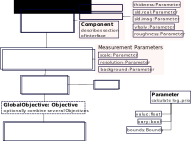
\includegraphics[width=85mm]{components.pdf}
  \caption{Schematic showing the relationship between classes that make up a typical reflectometry curve-fitting problem. The key step for the user is assembling materials (\Component) such as a `Slab: Component' (a \Component\ that is a \Slab) and encoding prior knowledge into each \Parameter\ that describes that \Component.}
  \label{fig:components}
\end{figure}

The building block of the analysis is the \Parameter\ object which represents a model value (e.g. the SLD of the material), whether it is allowed to vary in a fit, and a bounds attribute. The bounds are a probability distribution representing pre-existing knowledge of a parameter's value, called a prior probability.
A prior might be a simple uniform distribution that specifies a lower and upper bound (e.g. volume fraction is in the interval $[0, 1]$), or a normal distribution that represents an experimentally derived value and associated uncertainty (e.g. thickness is $\SI{100+-4}{\angstrom}$).
Any of the \emph{scipy.stats} \cite{Jones2001-2017} continuous distributions, or other distributions created by the user, can be used for this purpose. Algebraic relationships between \Parameter\ objects can be applied to permit more sophisticated constraints that can cross between \Component\ objects (e.g. the sum of the thicknesses of several layers is known to some uncertainty).

\subsection{Structure representation}

The \Structure\ object represents the interfacial model, assembled from individual \Component\ objects in series. Each \Component\ represents a subset of the interface and selected attributes of the \Component\ can be described by physically relevant \Parameter\ objects. The simplest and most familiar \Component\ is a \Slab, which has a uniform scattering length density (SLD), thickness, roughness, and volume fraction of solvent. The simplest models are simply a series of \Slab\ objects.
More sophisticated components include \LipidLeaflet\ (a lipid monolayer, or one-half of a lipid bilayer) and \Spline\ (for free-form modelling of an SLD profile using spline interpolation).
It is straightforward to develop/modify new components for different structural functionality, a consequence of the program design.

To include further prior knowledge of the real sample into the model,
each \Component\ can additionally contribute to the prior probability in addition to its constituent \Parameter\ objects. This is useful when a \Component\ has a derived value, such as surface excess, which is already known.

To calculate the reflectivity from series of \Component\ objects that form the model,
each \Component\ has a \emph{slabs} property that represents a discretised `slice' approximation to a continuous SLD profile for its particular region of the interface. A \Slab\ object has a single slice because it is a single thickness of uniform SLD. A \LipidLeaflet\ is made of two slices (head/tail regions), but the \Spline\ has many thin slices approximating the smooth curve. Each of these slices has uniform SLD, with the N\'{e}vot--Croce approach being used to describe the roughness between them \cite{Nevot1980}.

The \Structure\ object is used to construct a \ReflectModel\ object. This object is responsible for calculating the resolution smeared reflectivity of the \Structure, scaling the data, and adding a $Q$-independent constant background (via the scale and background \Parameter\ objects). There are different types of smearing available: constant $\mathrm{d}Q/Q$, point-by-point resolution smearing read from the dataset of interest, or via a smearing probability kernel of arbitrary shape \cite{Nelson2014}. The constant $\mathrm{d}Q/Q$ and point-by-point smearing use Gaussian convolution, with $\mathrm{d}Q$ representing the full width half maximum (FWHM) of a Gaussian approximation to the instrument resolution function \cite{Well2005}.

\subsection{Model/data comparison}
The \Objective\ class is the comparator of the predicted and measured reflectivities, using the \ReflectModel\ and a dataset, \DataD, to calculate $\chi^2$, log-likelihood (Equation~\ref{eqn:2}), log-prior, residuals, and the generative model.
The \DataD\ object has \emph{x, x\_err, y, y\_err} attributes to represent $Q$, $\mathrm{d}Q$, $R$, $\mathrm{d}R$. As is standard for many reflectometry data files, the \DataD\ object reads a three or four column plain-text datafile. A three column dataset represents $Q$ (\si{\per\angstrom}), $R$, $\mathrm{d}R$ (1 standard deviation). A four column dataset represents $Q$ (\si{\per\angstrom}), $R$, $\mathrm{d}R$, $\mathrm{d}Q$ (\si{\per\angstrom}).
$\mathrm{d}R$ is the uncertainty in reflectivity, and $\mathrm{d}Q$ specifies the FWHM of the instrument resolution function, for each datapoint.
Extending \DataD\ would allow other formats to be read - at the moment there is no standardised data format for reflectometry.  One example of this could be a wavelength dispersive file using ($\Omega$, $\lambda$)-data instead of $Q$, such as that used in energy scanned X-ray reflectometry, or sometimes produced by wavelength dispersive neutron reflectometers. In such a case \ReflectModel\ could be subclassed to make full use of this energy dispersive information.
Creation of a standardised data format for reflectometry would facilitate ingestion of data, and allow other important information, such as experimental metadata, to be used.

An \Objective\ can be given a \Transform\ object to permit fitting as $\log_{10} R$ vs $Q$, $RQ^4$ vs $Q$; the default (no \Transform) is $R$ vs $Q$. Several \Objective\ objects can be combined to form a \GlobalObjective\ for co-refinement. The object-oriented nature allows reuse of \Parameter and \Component\ objects, and this is the basis for linking parameters between samples for co-refinement. For a comprehensive demonstration of multiple contrast co-refinement, see the annotated notebook in the supporting information.

\subsection{Statistical comparison and model refinement}

The \Objective\ statistics are used directly by the \CurveFitter\ class to perform least-square fitting with the functionality provided by the \SciPy\ package (Differential  Evolution, Levenberg--Marquardt, LBFGSB - Limited Broyden--Fletcher--Goldfarb--Shanno with bounds). Additional \SciPy\ solvers can be added relatively simply and it would be possible for other minimisers to use \Objective\ directly.
\CurveFitter\ can also perform Bayesian Markov Chain Monte Carlo (MCMC) sampling of the system, examining the posterior probability distribution of the parameters, Equation~\ref{eqn:1}. The posterior distribution is proportional to the product of the prior probability and the likelihood (or the sum of the log-probabilities):
%
\begin{gather} 
\label{eqn:1}\ p(\theta | D, I) = \frac{p(\theta | I)\times p(D | \theta, I)}{p(D | I)}\\
p(D | \theta, I) = -\frac{1}{2} \sum_n \left[\left(\frac{y_n - y_{\mathrm{model},n}} {\sigma_n}\right)^2 + \log(2\pi\sigma_n^2)\right]\label{eqn:2}
\end{gather}
%
The prior, $p(\theta | I)$, is the probability distribution function for a parameter, $\theta$, given pre-existing knowledge of the system, $I$, as outlined above.
The likelihood (Equation~\ref{eqn:2}), $p(D | \theta, I)$, is the probability of the observed data, $D$, given the model parameters and other prior information. It is calculated from the measured data, $y_n$ (with uncertainties $\sigma_n$), and the generative model, $y_{\mathrm{model},n}$. The likelihoods that are used here assume that the measurement uncertainties are normally distributed, Equation~\ref{eqn:2}. However, other types of measurement uncertainties (e.g. Poissonian) could be implemented by a subclass of \Objective\ overriding the log-likelihood method.
The model evidence, $p(D | I)$, is a normalising factor.

The posterior probability, $p(\theta | D, I)$, describes the distribution of parameter values consistent with the data and prior information. In the simplest form, this is akin to a confidence interval for a parameter derived by least-squares analysis. However, when parameters are correlated, or two models give similar quality of fit (`multi-modality'), a simple confidence interval can be misleading.
The posterior probability is derived by encoding the likelihood and prior distributions and then using an MCMC algorithm (via the \emcee\ and \ptemcee\ packages) to perform affine invariant ensemble sampling \cite{emcee, ptemcee}.
At the end of an MCMC run, the parameter set possesses a number of samples (called a `chain'); the samples reveal the distribution and covariance of the parameters, the spread of the model-predicted measurements around the data, and in a reflectometry context, the range of SLD profiles that are consistent with the data.
The chain statistics are used to update each \Parameter\ value, and assign a standard uncertainty. For the sampling, these represent the median and half the $[15.87, 84.13]$ percentile range respectively; the latter approximating the standard deviation for a normally distributed statistic.

The \ptemcee\ package is a variant (a `fork' in open-source software development terms) of the \emcee\ package that has been extended to implement the parallel tempering algorithm for characterisation of multi-modal probability distributions; different modes can be traversed by chain populations at higher `temperatures', while individual modes are efficiently explored by chains at lower `temperatures' \cite{ptemcee}.  Having multiple populations in the parallel tempering algorithm allows the sampler to escape local maxima, greatly aiding it's ability to explore the most probable regions of the posterior.  \ptemcee\ is also able to estimate the log-evidence term (the denominator in Equation~\ref{eqn:2}), which is useful when calculating the Bayes factor for model comparison.

Parallelisation of the sampling is automatic, making full use of multi-core machines, and can use MPI on a cluster for yet greater parallelisation. Visualisation of the samples produced by MCMC sampling is performed using the \corner\ package for scatter plot matrices \cite{corner}, which gives a representation of the probability distribution function for each individual parameter and also the covariance for each pair of parameters. As will be seen later, the plot for two normally distributed and uncorrelated parameters is isotropic, while covariant parameters show significant anisotropy. An evaluation of the impact of hard bounds can also be made by looking for plots where the bounds are clearly truncating the distribution function, allowing the bounds to be re-evaluated and adjusted if necessary.

\subsection{User interface}

A significant motivation in the development of \refnx\ has been the facilitation of reproducible analysis by helping the user describe \emph{how} the analysis was performed. A few lines of computer code is an incredibly powerful description, conveying the details with precision that is hard to match in written text, as well as being incredibly concise.
Example analyses within the \refnx\ code base are often sufficient to complete the task.
These few lines of Python code can be further extended to produce publication quality plots saved and ready to import into the next publication, or used in a loop for batch fitting purposes.
While Python is a popular language for instruction and for data analysis, meaning that the relatively few lines of code required to complete a \refnx\ analysis of a set of experiments is not a huge hurdle, a simpler graphical user interface (GUI) is also provided.
The browser-based GUI is available for fitting within a \Jupyter\ notebook, Figure~\ref{fig:gui}, leveraging the \ipywidgets\ modules \cite{ipywidgets}. The GUI has a `To code' button that turns the current model into the few lines of code required to perform the analysis without using the GUI, thus providing the desired instructions for the reproducible analysis. The ability to generate analysis code allows also makes it a stepping point for building more advanced models independently.
The current GUI is able to use slab based models for fitting a single dataset; a fully functional web-based reflectometry analysis notebook is currently available \cite{Nelson2018}.
If desired, it is possible to execute Jupyter notebooks in batch mode or to run the generated Python code within a Python program to complete batch mode fitting of larger data sets. The \refnx\ repository contains a growing set of examples of different uses of the \refnx\ package.

\begin{figure}
  \includegraphics[width=85mm]{./supporting_information/gui.png}
  \caption{Screenshot of the \Jupyter/\ipywidgets\ GUI; this \Jupyter\ notebook is available in the supporting information.}
  \label{fig:gui}
\end{figure}

\section{Example data analysis with a lipid bilayer}

Neutron reflectometry is an ideal technique for the study of biologically relevant lipid membrane mimics and their interactions with proteins, etc. Multiple contrast variation measurements are necessary to reduce modelling ambiguity (due to loss of phase information in the scattering experiment) and improve the ability to determine the structure of various components in the system. The gold standard approach for analysis of these datasets is co-refinement with a common model, and to parameterise the model in terms of chemically relevant parameters, such as the area per molecule \cite{campbell2018}. Sometimes a patchy coverage (distinct to low area per molecule) necessitates the use of an (incoherent) sum of reflectivities from different areas. \refnx\ has functionality for all these requirements, such as the \LipidLeaflet\ component for describing the head and tail groups of a lipid leaflet, and \MixedReflectModel\ to account for patchiness.

The parameters used in the \LipidLeaflet\ component are: area per molecule ($A$), thicknesses for each of the head and tail regions ($t_x$), sums of scattering lengths of the head and tail regions ($b_x$), partial volumes of the head and tail groups ($V_x$), roughness between head and tail region, and SLDs of the solvents for the head and tail group ($\rho_{x,\mathrm{solv}}$). The overall SLD of each of the head and tail group regions are given by:
\begin{gather} 
\label{eqn:3} \phi_{x} = \frac{V_x}{At_x}\\
\rho_x =  \phi_{x} \frac{b_x}{V_x} + (1 - \phi_{x})\rho_{x,\mathrm{solv}} \label{eqn:4}
\end{gather}
The approach used in \LipidLeaflet\ component ensures that there is a 1:1 correspondence of heads to tails.
By default the head and tail solvents are assumed to be the same as the solvent that is used throughout the \Structure. This will be the case when using \LipidLeaflet\ for a solid-liquid reflectometry experiment. However, at the air-liquid, or liquid-liquid interfaces the solvent for the head and tail region may be different, and it is possible to use different solvent SLDs for each. We note that the \LipidLeaflet\ component may also be used to describe other amphiphiles adsorbing at an interface.

Here, \LipidLeaflet\ is used to co-refine three contrasts (\ce{D_2O}, \ce{Si} contrast match [hdmix, SLD=\SI{2.07E-6}{\per\square\angstrom}], and \ce{H_2O}) of a 1,2-dimyristoyl-sn-glycero-3-phospho\-choline (DMPC) bilayer at the solid-liquid interface, Figure~\ref{fig:global_fit}.\footnote{The validity of \LipidLeaflet\ does depend on the area per molecule being equal for the headgroup and tailgroup regions, as pointed out by Gerelli \cite{Gerelli2016}, which can be violated if there are guest molecules that insert in the membrane.} Two \LipidLeaflet\ objects are required to describe the inner and outer leaflets of a bilayer, hence, the component contains an attribute which can reverse the direction of one of the leaflets. The use of individual objects to describe each leaflet leads to great flexibility; it becomes easy to model asymmetric bilayers (inner leaflet can be a different lipid to the outer lipid), and one can model interstitial water layers between the leaflets as well.

The \Jupyter\ notebook used for the analysis, \emph{lipid.ipynb}, is available in the supporting information. The corner plot (Figure~\ref{fig:corner}) produced from the MCMC analysis shows the covariance between parameters, with an area per molecule of \SI{57.0 \pm0.15}{\square\angstrom}. Figure~\ref{fig:global_fit} shows the probability distribution of the generative model around the data and in the SLD profile. These families of plausible fits that are obtained by plotting a subset of samples from the MCMC chain. The spread in SLD profiles is used to determine what range of structures is consistent with the data. Multi-modalities in these SLD profiles can be due to statistical uncertainties, the $Q$ ranges measured, and the loss of phase information in NR \cite{Majkrzak1999, Heinrich2009}.

\begin{figure}
\centering
\label{fig:global_fit}%
\includegraphics[width=100mm]{./supporting_information/global_fit.pdf}%


\includegraphics[width=100mm]{./supporting_information/d2o_sld_spread.pdf}

\caption{a) Neutron reflectivity from a DMPC bilayer supported on a silicon crystal, measured at three contrasts, with 500 samples from the posterior distribution in grey and median of the distribution in red. Data for the contrast matched (HD\textsubscript{mix}) and \ce{H2O} contrast offset by 0.1 and 0.01 respectively. b) SLD profile of the \ce{D2O} model showing 500 samples from the posterior distribution, as well as the median in red. It is seen that the uncertainty in the reflectivity at high $Q$ is associated with an uncertainty in SLD profile at the lipid-\ce{D2O} interface.}
\end{figure}

\begin{figure}
  \includegraphics[width=120mm]{./supporting_information/corner.pdf}
  \caption{Corner plot for the varying parameters of DMPC bilayers supported on a silicon crystal, measured at three contrasts. The sampling took $\sim$\SI{33}{\minute} on a \SI{2.8}{GHz} quad-core computer for 20 saved steps, corresponding to 4000 samples, with the steps being thinned by a factor of 400. A larger scale image is available in supporting information.}
  \label{fig:corner}
\end{figure}

 
\section{Distribution and Modification}

Each submodule in \refnx\ possesses its own unit testing code for checking that the functions and classes in the module operate correctly, both individually and collectively. For example, there are tests that check that the reflectivity of a model is calculated correctly, or that the behaviour of a function is correct for the different possible inputs and code paths through it. Since the test suite is an integral part of the package each installation is testable. In addition, there is a benchmarking suite to track changes in performance, specifically the speed of critical calculations, over time. This development approach is important to providing assurances to the community that the code is tested and works.

The source code for \refnx\ is held in a publicly accessible version controlled git repository \cite{refnx}. User contributions may be made using the standard GitHub workflow in which contributors create their own `fork' of the main \refnx\ repository, and create a feature branch to which they make modifications.
They then submit a pull request (PR) against the main repository. The modifications made in the PR are checked on continuous integration (CI) web-services that run the test suite against a matrix of Python versions on the macOS, Linux and Windows operating systems. Features are merged into the main repository if all tests pass, and if manual code review concludes that the changes are scientifically correct, of sufficiently high standard, and useful. When a sufficient number of features have accumulated, a new release is made. Successive releases have an incrementing semantic version number which can be obtained from the installed package, with each release being given its own Digital Object Identifier (DOI).
We encourage users to submit models for inclusion in a user-contributed models repository (refnx-models\footnote{https://github.com/refnx/refnx-models}). We will work with users to develop a suitable way of documenting and sharing their models.

The recommended way of using \refnx\ is from a \conda\ environment, which offers package, dependency and environment management \cite{conda}, using the pre-compiled distributables on the \refnx\ conda-forge channel. These distributables are made as part of the release process using the same CI web-services used to test the code. The matrix of distributables covers the major Python versions currently in use, across the macOS, Windows, and Linux operating systems. Alternatively the package can be installed from source, either directly from the git repository, or via \pip\ from the version uploaded to PyPI.\footnote{https://pypi.python.org/pypi/refnx; the installation command is `\texttt{pip install refnx}'} Building from source requires a C compiler and the \Cython\ and \NumPy\ packages to be installed; further dependencies should be installed to run the test suite to verify that compilation and installation was successful.

\refnx\ is released under the BSD permissive open source licence. In addition, all of the  dependencies of \refnx\ are released under open source licences which means that use is free of cost to the end user and, more importantly, the user is free to modify, improve, and inspect this software.

\section{Comments on reproducibility of analyses}

In order for a given scattering analysis to be fully reproducible by others, a general set of conditions need to be met \cite{Helliwell2017, Moeller2017a}:
\begin{itemize}
  \item the processed datasets used in the analysis need to be deposited with a journal article, or be freely available. Ideally the raw datasets, and the means to create the processed datasets should also be made available.
  \item the exact software environment needs to be recreatable.
  \item the exact ordered set of steps taken during the analysis needs to be listed.
\end{itemize} 
Each of these points is often inadequately addressed in the literature. For example, the use of different software versions may change the output of an analysis, or the use of a GUI program may preclude recording the full set of steps, or options, applied by a user \cite{Chirigati2013}. Whilst it is unable to meet the first criterion by itself, the use of \refnx\ in a \Jupyter\ notebook can fulfil the other two requirements, providing a little care is taken. As we have already noted, the ordered set of steps to perform the analysis is the \Jupyter\ notebook in which the analysis was performed and this is an artefact able to be archived.

The exact software environment can be recreated by noting down the versions of the software packages used during an analysis (\refnx, \SciPy, \NumPy, Python, etc). At a later date those exact versions can be installed in the same Python version using one of: the \conda\ package manager, by installing from the source at a given version tag in the git repository, or by \pip. \conda\ can use environment files to recreate a specific setup. An alternative way of recreating the environment is by using a virtual machine, or other container environment such as Docker; the strengths and weaknesses of various software distribution practices and the relationship with reproducible science has been discussed in detail elsewhere \cite{Moeller2017a}.

The usefulness of open-source software in a git (or other version controlled) repository must be emphasised here \cite{Moeller2017a}. With closed source or proprietary software, the ability to return to a specific software version/environment can be frustrated, and different versions can have modifications that can unknowingly change the output of an analysis. In addition reduced accessibility (due to cost, etc) to the wider scientific community can also hinder reproducibility.

Moreover, there are important ramifications for verifiability \cite{Chirigati2013}. \refnx\ is based on a fully open software stack, with good unit test coverage. The user can run tests for each component and inspect parts for correctness. For example, the behaviour of the reflectivity calculation in \refnx\ is checked from first principles in the test suite; and can be done now and in several years time. If problems are discovered, they can be corrected. With a fully or partially closed-source program such checking is much harder, as one does not possess full knowledge of what happens inside.

\section{Conclusions}\label{conclusions}

\refnx\ is a powerful tool for least-squares or Bayesian analysis of neutron and X-ray reflectometry data that is ideally usable for reproducible research with \Jupyter\ notebooks, and has been built with extensibility in mind. Its features include: MCMC sampling of posterior distribution for parameters, structural models constructed from modular components with physically relevant parameterisation, algebraic inter-parameter constraints, mixed area models, co-refinement of multiple datasets, probability distributions for parameter bounds used directly for log-prior terms, and a (\Jupyter) \ipywidgets\ GUI.

\section*{Acknowledgements:}
We acknowledge Anton Le Brun (ANSTO) for the provision of the lipid bilayer datasets in the example, James Hester (ANSTO) for comments made on the draft manuscript, and Andrew McCluskey (Bath University) and Isaac Gresham (UNSW) for important feedback on \refnx\ development.

\section{Supporting information}

\noindent
\textbf{gui.ipynb} - \Jupyter\ notebook used to create the GUI screenshot.\\
\textbf{lipid.ipynb} - \Jupyter\ notebook used for the lipid analysis example.\\
\textbf{lipid.pdf} - PDF view of the \Jupyter\ notebook used for the lipid analysis example.\\
\textbf{corner.pdf} - larger scale image of the corner plot.\\
\textbf{c\_PLP0016596.dat}, \textbf{c\_PLP0016601.dat}, \textbf{c\_PLP0016607.dat} - example lipid datasets.\\
\textbf{reduction.ipynb} - notebook for reducing example datasets.\\
\textbf{raw\_data.zip} - raw files for the example datasets.\\
\textbf{refnx-paper.yml} - \conda\ environment file to reproduce the analysis environment in this paper.

\bibliographystyle{abbrv}
\bibliography{main}
\end{document}
